\documentclass[tikz,border=6pt]{standalone}
\usepackage{pgfplots}
\pgfplotsset{compat=1.18}
\usepgfplotslibrary{colormaps}
\usetikzlibrary{arrows, arrows.meta, calc}
\usetikzlibrary{decorations.markings}


\usepackage{amssymb,amsmath,mathtools}

\usepackage[T1]{fontenc}
\usepackage[utf8]{inputenc}
\usepackage{newpxtext,newpxmath}
\usepackage{sectsty}

\renewcommand{\Re}{\operatorname{\mathrm{Re}}}
\renewcommand{\Im}{\operatorname{\mathrm{Im}}}

\begin{document}
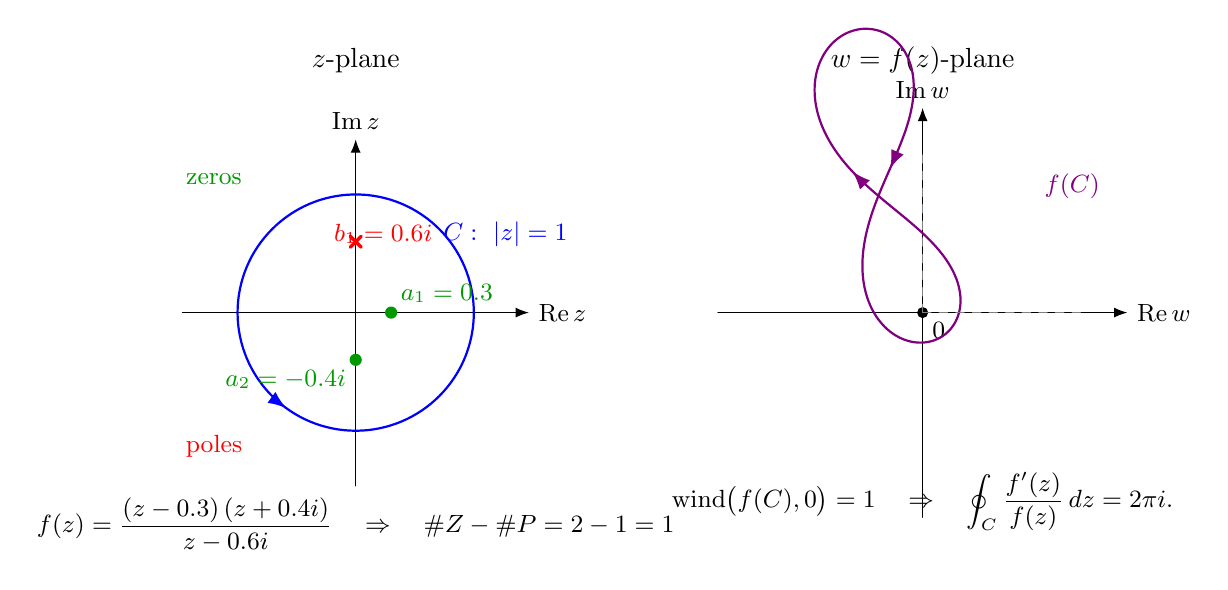
\begin{tikzpicture}[>=Latex, line cap=round, line join=round, font=\small]

%========================
% Left: z-plane
%========================
\begin{scope}[shift={(0,0)}]
	\node[font=\normalsize] at (0,3.2) {$z$-plane};
	% axes
	\draw[->] (-2.2,0)--(2.2,0) node[right] {$\Re z$};
	\draw[->] (0,-2.2)--(0,2.2) node[above] {$\Im z$};
	
	% unit circle C (positively oriented)
	\draw[blue,thick,postaction={decorate},
	decoration={markings, mark=at position 0.65 with {\arrow{>}}}]
	(0,0) circle (1.5);
	\node[blue] at (1.9,1.0) {$C:\ |z|=1$};
	
	% zeros inside C (green dots)
	\fill[green!60!black] (0.45,0) circle(2.2pt) node[above right] {$a_1=0.3$};
	\fill[green!60!black] (0,-0.6) circle(2.2pt) node[below left] {$a_2=-0.4i$};
	\node[green!60!black] at (-1.8,1.7) {zeros};
	
	% a pole inside C (red cross)
	\draw[red,very thick] (0,0.9) ++(-0.07,-0.07) -- ++(0.14,0.14);
	\draw[red,very thick] (0,0.9) ++(-0.07,0.07) -- ++(0.14,-0.14);
	\node[red] at (0.35,1.0) {$b_1=0.6i$};
	\node[red] at (-1.8,-1.7) {poles};
	
	% function label
	\node[align=left] at (0,-2.7) {$\displaystyle
		f(z)=\frac{(z-0.3)\,(z+0.4i)}{z-0.6i}\quad
		\Rightarrow\quad \#Z-\#P=2-1=1$};
\end{scope}

%========================
% Right: w-plane = f(z)-plane
%========================
\begin{scope}[shift={(7.2,0)}]
	\node[font=\normalsize] at (0,3.2) {$w=f(z)$-plane};
	% axes
	\draw[->] (-2.6,0)--(2.6,0) node[right] {$\Re w$};
	\draw[->] (0,-2.6)--(0,2.6) node[above] {$\Im w$};
	
	% origin
	\fill (0,0) circle(2pt) node[below right] {$0$};
	
	% image curve f(C): parametrize z = e^{it}, t in [0,2pi]
	% Let a+ib = e^{2it} = (cos 2t, sin 2t)
	% Let c+id = e^{it}-0.6i = (cos t, sin t - 0.6)
	% Multiply numerator by (z-0.3)(z+0.4i):
	% First form z = cos t + i sin t
	% We directly evaluate Re/Im using the real/imag algebra inside the plot.
	\draw[violet,thick,
	postaction={decorate},
	decoration={markings,
		mark=at position 0.18 with {\arrow{>}},
		mark=at position 0.62 with {\arrow{>}}}]
	plot[domain=0:6.283, samples=600] 
	({ % Re f(e^{it})
		% z = x+iy with x=cos t, y=sin t
		% N = (z-0.3)(z+0.4i) = (x-0.3 + i y)*(x + i(y+0.4))
		%   = [(x-0.3)x - y(y+0.4)] + i[(x-0.3)(y+0.4) + xy]
		%   = [x^2 -0.3x - y^2 -0.4y] + i[ x(y+0.4) -0.3(y+0.4) + xy]
		% D = z - 0.6i = x + i(y-0.6)
		% Re = (ReN*ReD + ImN*ImD)/(|D|^2)
		% Im = (ImN*ReD - ReN*ImD)/(|D|^2)
		% Implement with x=cos(t), y=sin(t)
		( ( (cos(\x r)*cos(\x r) - 0.3*cos(\x r) - sin(\x r)*sin(\x r) - 0.4*sin(\x r)) * cos(\x r)
		+ ( (cos(\x r)*(sin(\x r)+0.4) - 0.3*(sin(\x r)+0.4) + cos(\x r)*sin(\x r)) * (sin(\x r)-0.6) )
		)
		/
		( cos(\x r)*cos(\x r) + (sin(\x r)-0.6)*(sin(\x r)-0.6) )
	},
	{ % Im f(e^{it})
		( ( (cos(\x r)*(sin(\x r)+0.4) - 0.3*(sin(\x r)+0.4) + cos(\x r)*sin(\x r)) * cos(\x r)
		- ( (cos(\x r)*cos(\x r) - 0.3*cos(\x r) - sin(\x r)*sin(\x r) - 0.4*sin(\x r)) * (sin(\x r)-0.6) )
		)
		/
		( cos(\x r)*cos(\x r) + (sin(\x r)-0.6)*(sin(\x r)-0.6) )
	});
	
	\node[violet] at (1.9,1.6) {$f(C)$};
	
	% dashed rays to visualize winding
	\draw[gray,dashed] (0,0) -- (2.1,0);
	\draw[gray,dashed] (0,0) -- (0,2.1);
	
	% annotation
	\node[align=center] at (0,-2.4)
	{$\displaystyle \mathrm{wind}\big(f(C),0\big)=1
		\quad\Rightarrow\quad
		\oint_C \frac{f'(z)}{f(z)}\,dz=2\pi i.$};
\end{scope}

\end{tikzpicture}
\end{document}
